\documentclass[11pt]{article}
\usepackage[margin=1in]{geometry}
\usepackage{amsmath,amssymb,booktabs,graphicx,hyperref,xcolor}
\newcommand{\pending}[1]{\textcolor{red}{[PENDING: #1]}}
\newcommand{\fro}{\mathrm{F}}
\title{What does Dimuon do to a LoRA?\\ \large A black-box measurement study of an undocumented optimizer}
\author{Working draft --- updated as experiments complete. Status line: see Section~\ref{sec:status}.}
\date{Started 10 November 2026}
\begin{document}
\maketitle

\begin{abstract}
Dimuon is an optimizer for LoRA fine-tuning offered on the Tinker API. Its documentation gives
three hyperparameters and usage guidance but not the update rule. We measure the rule from the
outside: we take single optimizer steps on small LoRA adapters, export the adapter weights before
and after, and compare the observed update with the gradient, which we recover separately.
\pending{headline findings once the first-step law, the momentum law and the A/B coupling are
measured and cross-checked.}
\end{abstract}

\section{Status of this draft}\label{sec:status}
Everything in black has been measured or is sourced as stated. Red text marks claims that are
planned but not yet supported by data. The lab journal with every run is
\texttt{dimuon/experiments.md}.

\section{Background, from the ground up}

\subsection{Gradient descent and the question every optimizer answers}
Training minimises a loss $L(W)$ over weights $W$. The gradient $G=\partial L/\partial W$ says how
the loss changes for an infinitesimal change in each weight. Plain gradient descent moves against
it, $W \leftarrow W-\eta G$, with learning rate $\eta$. The gradient gives a \emph{direction}; it
does not say how far it is safe to go, and its entries can differ in size by orders of magnitude
across a network. Every practical optimizer is an answer to one question: \emph{given $G$ (and its
history), what step $\Delta W$ should be taken?} Different answers correspond to different notions
of what a ``unit-size'' step is.

\subsection{Momentum}
Minibatch gradients are noisy. Momentum averages them over time,
$M_t=\beta M_{t-1}+(1-\beta)G_t$ (one common convention), and steps along $M_t$. With
$\beta=0.9$ the average covers roughly the last ten gradients.

\subsection{Adam and AdamW: per-entry normalisation}
Adam keeps the momentum $m_t$ and a second running average $v_t$ of the squared gradient, and
steps each weight by
\[
\Delta w = -\eta\,\frac{\hat m_t}{\sqrt{\hat v_t}+\epsilon},
\]
where the hats denote the standard correction for the averages starting at zero. Each entry is
divided by its own typical magnitude, so every weight moves about $\eta$ per step regardless of how
large its gradient is. On the very first step $\hat m_1=g$ and $\hat v_1=g^2$, so
$\Delta w=-\eta\, g/(|g|+\epsilon)$: with tiny $\epsilon$ this is $-\eta\,\mathrm{sign}(g)$, and
with large $\epsilon$ it is proportional to $g$. We use the second fact as a measuring instrument
(Section~\ref{sec:oracle}). AdamW adds weight decay applied directly to the weights. Adam treats a
weight matrix as a bag of unrelated numbers: it is blind to the fact that the matrix acts as a
linear map.

\subsection{Muon: per-direction normalisation}
A matrix $G\in\mathbb{R}^{m\times n}$ has a singular value decomposition $G=USV^\top$: orthonormal
input directions (columns of $V$), orthonormal output directions (columns of $U$), and
non-negative strengths $S$. Muon~\cite{jordan2024muon} takes the momentum matrix and replaces it
by $UV^\top$, i.e.\ it sets every singular value to one. This is the nearest semi-orthogonal
matrix to $G$ in Frobenius norm. Where Adam equalises the step \emph{per entry}, Muon equalises it
\emph{per direction}. Jordan's stated motivation is empirical: updates for transformer weight
matrices ``typically have very high condition number'' --- a few directions dominate --- and
orthogonalising boosts the rare directions.

Computing an SVD every step is expensive, so Muon approximates $UV^\top$ with a Newton--Schulz
iteration: normalise $X_0=G/\|G\|_\fro$ and repeat $X\leftarrow aX+b(XX^\top)X+c(XX^\top)^2X$,
which applies the odd polynomial $\varphi(x)=ax+bx^3+cx^5$ to every singular value while leaving
$U$ and $V$ untouched. Muon uses $(a,b,c)=(3.4445,-4.7750,2.0315)$ for five steps in bfloat16.
These coefficients are tuned for speed, not exactness: the singular values end up \emph{near} one,
in a band, rather than exactly at one. That band is a fingerprint an outside observer can look for.

\subsection{LoRA and why it complicates the picture}
LoRA freezes a pretrained weight $W_0\in\mathbb{R}^{d_\text{out}\times d_\text{in}}$ and trains a
low-rank correction $W=W_0+\tfrac{\alpha}{r}BA$ with $B\in\mathbb{R}^{d_\text{out}\times r}$ and
$A\in\mathbb{R}^{r\times d_\text{in}}$, $r\ll d$. $B$ starts at zero so training begins exactly at
the pretrained model. By the chain rule, with $G_W=\partial L/\partial W$,
\[
G_B=\tfrac{\alpha}{r}\,G_W A^\top,\qquad G_A=\tfrac{\alpha}{r}\,B^\top G_W .
\]
Two consequences matter here. First, at initialisation $B=0$ so $G_A=0$: on the first step only
$B$ can move. Second, the factorisation is not unique: $(BQ^{-1})(QA)$ is the same adapter for any
invertible $Q$, but the gradients, and therefore the steps of an optimizer applied to $A$ and $B$
separately, change with $Q$. An optimizer ``built for LoRA'' has to take some position on this:
it may treat $A$ and $B$ as two unrelated matrices, or use the structure of the product. Which one
Dimuon does is one of our questions.

\section{What is publicly documented}
The Tinker documentation\footnote{\url{https://tinker-docs.thinkingmachines.ai/tinker/optimizers/},
read 10 Nov 2026.} describes Dimuon as an in-house optimizer built for LoRA fine-tuning, selected
at client creation, with per-step parameters \texttt{learning\_rate} (required; ``typically
10--100$\times$ AdamW's''), \texttt{beta1} (default 0.9, a momentum coefficient) and
\texttt{grad\_clip\_norm} (default off). It reports that in the authors' supervised fine-tuning
runs about $15\times$ the AdamW learning rate worked best and that Dimuon benefited more from
higher LoRA rank. It does not give the update rule.

\section{Method}
\subsection{Observing a step}
The SDK exports adapter weights in PEFT format as float32. We export, take one
\texttt{forward\_backward} and one \texttt{optim\_step} on a fixed short batch, and export again;
the difference is the update. All runs use Qwen3.5-4B unless stated.

\subsection{Recovering the gradient}\label{sec:oracle}
To compare an update with the gradient that caused it we need the gradient, which the API does
not return. We read it off AdamW. From a fresh optimizer state the first AdamW step is
$\Delta w=-\eta\,g/(|g|+\epsilon)$ per entry, which inverts exactly:
$|g|=\epsilon|\Delta w|/(\eta-|\Delta w|)$, $\mathrm{sign}(g)=-\mathrm{sign}(\Delta w)$. A second
client with the same seed and batch, run for one AdamW step with $\eta=1,\epsilon=100$, therefore
yields $G$. We checked the formula rather than assumed it: seven settings of
$(\eta,\epsilon,\beta_1,\beta_2)$ recover gradients that agree to relative error
$6\times10^{-8}$--$2\times10^{-6}$, and the alternative $\sqrt{g^2+\epsilon}$ form fails by factors
of 2--30. The recovered values sit on an 8-significant-bit grid: the server computes gradients in
bfloat16. After snapping to that grid all seven settings give bit-identical $G$
(0 of 3{,}670{,}016 entries differ). One consequence: gradients are not exactly linear in the loss
scale ($\times 2$ is exact, $\times 10$ changes the direction by about $1.3\%$), so every run at a
different loss scale gets its own oracle run.

\subsection{Noise floor}
Initialisation is deterministic in the seed and independent of the optimizer: all 152 $A$
tensors are bit-identical across six clients, and $B=0$. Repeating the same Dimuon step in three
separate clients gives bit-identical weights. The measurement therefore has no sampling noise;
any gap between a hypothesised rule and the data is model error or finite-precision arithmetic.

\section{Results}
\subsection{Pilot: one step, rank 4}
One Dimuon step at $\eta=10^{-3}$ on a rank-4 attention-only adapter (304 tensors) left every
$A$ exactly unchanged, consistent with $G_A=0$ at $B=0$. Every $B$ update had Frobenius norm
$\approx 1.39\times10^{-3}$ independent of $d_\text{out}\in\{1024,\dots,8192\}$, with four singular
values close to but not equal to each other (e.g.\ $7.37,7.31,6.98,6.06\times10^{-4}$). A
width-independent norm with a near-flat spectrum is what an orthogonalising update produces; the
spread in the singular values is what remains to be explained.

\subsection{The first-step law}
Dataset D1: ranks $r\in\{1,2,4,8,16,32,64\}$, 152 attention modules each, the exact gradient $G_B$
and the one-step update $U$.

\paragraph{Step size.} For every tensor at every rank
\[
\|U\|_\fro=\eta\,\sqrt{r}\,(r/32)^{0.175}
\]
to within $\pm1.3\times10^{-7}$ relative. It depends on neither the layer width nor the size of the
gradient. $\sqrt r$ is the Frobenius norm of a matrix with $r$ unit singular values; the extra
factor $(r/32)^{0.175}$ is an explicit rank-dependent rescale (it equals one at $r=32$) whose
origin we measure but do not explain.

\paragraph{Direction.} $U$ is a spectral function of $G$: in the singular basis of $G$ it is
diagonal up to rounding, and all 19{,}304 singular values across ranks and modules fall on one
transfer curve when the input is normalised as $s_i/\|G\|_\fro$. No row or column scaling and no
dependence on $A$ is detectable at step one. The curve is linear below $x\approx10^{-3}$ and then
oscillates between about $0.875$ and $1.12$ (Figure~\ref{fig:transfer}). It is \emph{not} Muon's
fixed quintic. It is reproduced by five steps of a quintic iteration with a different coefficient
triple at each step --- the schedule we recognise as ``Polar Express''
\pending{verify the coefficients against the primary source; they were entered from memory and
selected by the data} --- with a safety factor of $1.01$ applied to both the input normalisation
and the coefficients. Table~\ref{tab:fs} shows what each ingredient buys.

\begin{table}[h]\centering\small
\begin{tabular}{lrrrrrrr}\toprule
rule & $r{=}1$ & 2 & 4 & 8 & 16 & 32 & 64\\\midrule
exact polar factor & 5.1e-4 & 4.4e-2 & 7.4e-2 & 8.2e-2 & 8.5e-2 & 4.9e-1 & 7.2e-1\\
Muon quintic, 5 steps & 5.1e-4 & 1.7e-1 & 1.8e-1 & 1.9e-1 & 2.0e-1 & 2.2e-1 & 2.3e-1\\
5-step schedule, no safety factor & 5.1e-4 & 6.5e-2 & 1.1e-1 & 1.1e-1 & 9.8e-2 & 1.0e-1 & 1.0e-1\\
5-step schedule, factor 1.01 & 5.1e-4 & 6.5e-3 & 6.5e-3 & 5.2e-3 & 9.6e-3 & 3.1e-2 & 4.0e-2\\
\quad + input rounded to fp16 & 4.6e-4 & 6.6e-3 & 6.5e-3 & 5.2e-3 & 5.6e-3 & 1.4e-2 & 1.8e-2\\\bottomrule
\end{tabular}
\caption{Median over 152 modules of $\|\hat U-U\|_\fro/\|U\|_\fro$ for candidate first-step rules.
The coordinator re-derived rows 1, 2 and 4 at $r\in\{2,8,32\}$ with independent code and obtained
the same values.}\label{tab:fs}
\end{table}

\begin{figure}[h]\centering
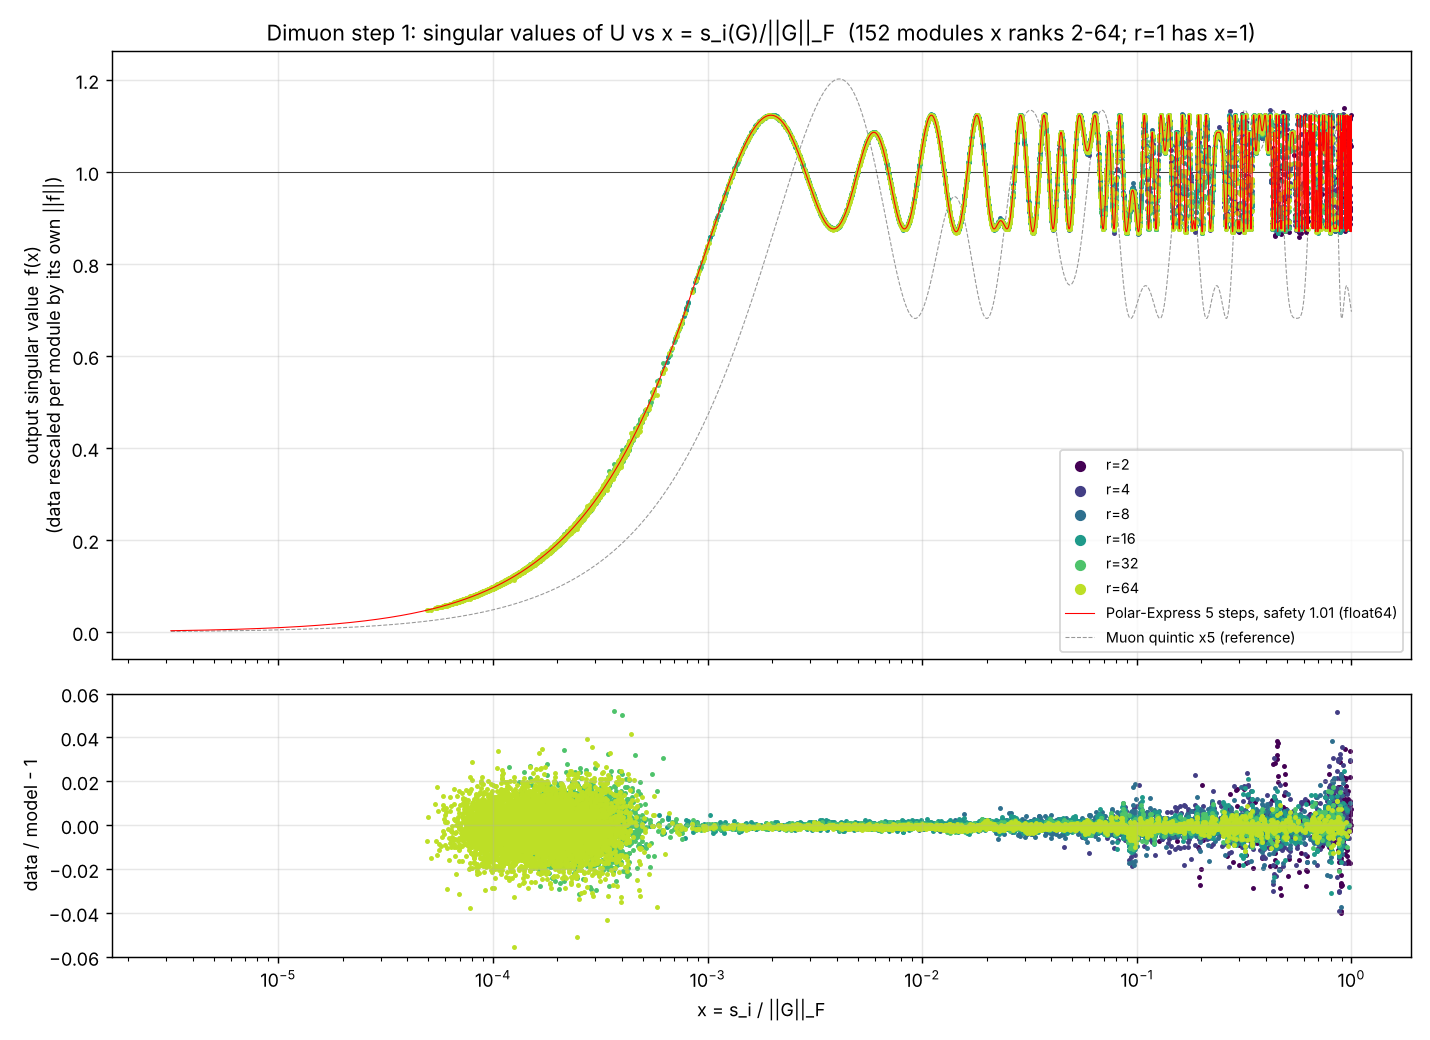
\includegraphics[width=.8\linewidth]{../figures/fs_transfer_function.png}
\caption{Measured transfer function: output singular value against normalised input singular
value, all ranks and modules.}\label{fig:transfer}
\end{figure}

\paragraph{Precision.} Every entry of every $U$ is one float32 scalar times an exactly
half-precision (fp16, 11 significant bits) number: the orthogonalisation runs in fp16, not the
bfloat16 that Muon uses. The remaining $0.5$--$2\%$ residual is consistent in size and location
with fp16 rounding inside the iteration; it is not reproduced bit-for-bit, and at ranks 2--16 the
server deviates from the ideal rule 1.5--2$\times$ more than our emulation's rounding does. That
excess is unexplained.

\paragraph{Momentum at step one.} $\beta_1=0$ and $0.5$ give bit-identical updates; $\beta_1=0.9$
differs in five entries of one tensor. A plain average $(1-\beta)G$ in float32 would change far
more entries, so it is rejected; a bias-corrected average is consistent. Step one cannot settle
this; the multi-step data will.
\subsection{Dependence on rank, learning rate and gradient scale}
The update is linear in $\eta$ to $5\times10^{-8}$ relative across $\eta\in[10^{-4},10^{-1}]$. It is
invariant to the scale of the gradient: at loss weights $0.1$, $1$ and $10$ (each against its own
oracle) the rule above fits equally well ($5.3$, $5.2$, $4.9\times10^{-3}$). Rank enters only
through the step size and through how ill-conditioned the gradient is.
\subsection{Momentum and state across steps}\pending{}
\subsection{How $A$ is updated, and whether $A$ and $B$ are coupled}\pending{}
\subsection{Cross-check on a second model}\pending{}
\subsection{Comparison with a public reimplementation}\pending{done last, after our own rule is
fixed, so the measurement is independent.}

\section{Limitations}
A black-box study can show that a rule reproduces the observed updates on the inputs tested. It
cannot show that the rule is the implementation, and it says nothing about inputs not tested.
\pending{specific gaps.}

\begin{thebibliography}{9}
\bibitem{jordan2024muon} K.~Jordan et al. \emph{Muon: An optimizer for hidden layers in neural
networks}. 2024. \url{https://kellerjordan.github.io/posts/muon/}
\end{thebibliography}
\end{document}
